\RequirePackage{fix-cm} % load new fixes to latex
\documentclass{inc/mas}
% \makeindex
%\usepackage[firstpage]{draftwatermark} %uncomment to set document as draft

\usepackage{multirow}
\usepackage{moreverb}
\usepackage{url}

\pdfsubject{}
\keywords{}
\title{Laboration 1 }
\subtitle{Algorithms, TIN092/DIT600\\ Knapsack, exhaustive search \\ Group 25}
\affiliation{}
\pdfauthor{Anne-Katrin Krolovitch, Linda Nilsson}
\begin{document}
%\AddToShipoutPicture{{\BackgroundPic}} % uncomment to add a background image
\author{Anne-Katrin Krolovitch \\ 861022-8960\\ \mail{annekatr@student.chalmers.se}\\ \and
Linda Nilsson \\ 840703-4860 \\ \mail{nilind@ituniv.se}\\ \tabularnewline
}
\maketitle
\section{Explanation of the Algorithm} 
 \noindent The problem which needs to be solved is as follows: there are a number of objects, which all have a size and a value, and we have a knapsack which has a capacity. This means that it only can take a certain amount of objects. These objects should amount to a value that is as large as possible.\\

\begin{figure}[h!]
  \centering
      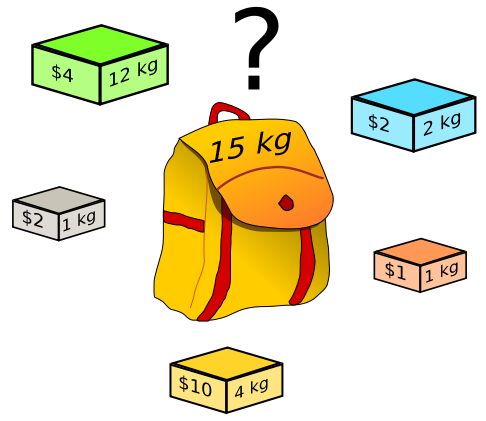
\includegraphics[width=0.5\textwidth]{Knapsack.png}
  \caption{An illustration of the Knapsack problem! \citep{wikipic} }
\end{figure}



\textbf{Measures:} The number of objects that are in the input file defined as n, and the number of possible subsets which can be created from them ($2^n$), defined as m are measured.\\

\noindent \textbf{Pseudocode:}
\begin{tabbing}
For \= all the objects in the input file \\
\> create \= power set	\\
\> select the best subset from the power set with the highest value\\
\end{tabbing}

After reading the input file and putting each of these objects into a Tuple which has a size and a value, the algorithm consists of two parts. First of all, the algorithm creates a power set (all possible subsets plus the set itself, see \citep{Gersting}) of the input Tuples, and second of all it selects the first subset which has a size less or equal to the capacity of the knapsack and has the highest value.\\
 

\section{Algorithm in Pseudocode}
In this chapter the algorithm will be explained in more detail. The following is the pseudocode for the function "createPowerset()". \newline

\begin{lstlisting}
n = Size of the tuple list 	
m = Size of possible subsets 2^n

for i = 0 to  m-1 loop
  element = 1  
  create temporary arraylist  
    for j = 0 to n-1 loop
       if (i "bitwise and" element is not 0)
         add tuple to temporary arraylist
       end if
       element = element << 1
    end for
    add subset to list
end for
\end{lstlisting}

\noindent This function creates a power set, which is a set of all possible subsets of the set and the set itself. It is known that the power set will have $2^n$ subsets. Through bit masking with the bitwise "and" operator and letting i = 1 to m represent all possible subsets, it is checked if the corresponding bits are both 1, in which case the current tuple is saved in a temporary array list. Using the shift left operator $<<$ the element is shifted one step to the left before next iteration to enable checking if the next element is part of the current subset. The final step before next iteration is to add the resulting subset to the list of subsets. Inspiration to the binary solution was taken from \citep{powerset}, section ``It's Binary``. \\ \\ 

The second part of the algorithm is to select the best possible subset and is shown in the pseudocode for function ``selectBestSet()``.\\

\begin{lstlisting}
k = Size of list containing all possible subsets
capacity = the capacity of the knapsack
bestValue = the best value of all subsets (intiated to 0)
bestSet = the set that gives bestValue

for i = 1 to k loop

  sumSizes = 0
  sumValue = 0

  for j = 1 to size of subset i loop
   store tuple j from subset i in tuple t
    add the size of the tuple t to sumSizes and store in sumSizes
    add the value of the tuple t to sumValue and store in sumValue
  end for

  if (sumSizes is less than or equal to the capacity)
    if(sumValue is greater than bestValue)
      store sumValue as bestValue
      store set i as bestSet
    end if
  end if
end for
\end{lstlisting}

\noindent This part of the algorithm is a greedy algorithm which chooses the best possible subset for the Knapsack problem, if several subsets produces equally good value the first such subset is selected. The function loops through all created subsets and adds up all sizes and values of the tuples in that subset. It then checks if the sum of the sizes is less than or equal to the capacity of the Knapsack and if it is it will check if the sum of the values of this subset is better than the previous bestValue. If a new bestValue was optained it will be stored as bestValue and also the subset giving this bestValue will be stored until the algorithm finds a subset which results in a better value.\\

\section{Correctness Justification}

The correctness of the algorithm is justified in two seperate sections, one for each part of the algorithm. For this the course litterature has been used for viewing examples of proofs \citep{Tardos}.

\subsection{Create powerset}
For the set $S = \{a,b,c\}$ a correct power set for S is $P = \{\{\},\{a\},\{b\},\{c\},\{a,b\},\{a,c\},\{b,c\},\{a,b,c\}$.

The createPowerset part of the algorithm has to make sure that each of the subsets in set $P$ are created. 

To do this, $n$ is defined as the number of elements in set $S$. In an execution of the algorithm the elements in $S$ would consist of tuples with a weight and size but here the tuples are represented by label $a,b$ and $c$.

The power set will have $2^n$ subset as shown in set $P$.\\\\

\textbf{Proof by contradiction}

Assume that the createPowerset part of the algoritm does not produce set $P$ when given the input of set $S$.

Letting the binary code for $i = 0$ to $2^n-1$ represent each possible subset, where a one in the binary code of $i$ means that the element from set $S$ at the place where the one is placed will be included and a zero means the element will not be included. For example, when $i = 5$ the binary code is 101 and the algorithm would include element $a$ and $c$ from the set $S$. By letting $element$ represent the placement of the element in set $S$ and setting $element = 1$, using a ''bitwise and'' compairison between $i$ \& $element$ where the result is $\neq0$ the element from set $S$ at place $element$ would be included in the subset. Since the algorithm for each $i$ iterates $n$ times, shifting the bit set to one in $element$ one step to the left compairing each binary code of $i = 0$ to $2^n-1$ with each element in set $S$ (represented by $elements$). Each possible subset will be created. A contradiction to our original assumption.

\subsection{Select best set}

\textbf{Proof by contradiction}

Assume that the selectBestSet does not select the best value among the subsets that fit in the knapsack.

Let $i = 0$ loop to $n$ where $n$ is the size of the subsetList and $j = 0$ loop through every object/Tuple in each subset $i$. For each object in a subset $i$ the algorithm stores the sum of the sizes and the sum of the values. It then compares if the size is $<=$ to the capacity, if so, the set would fit in the knapsack. When $i = 0$ it stores the first result of the values in $bestValue$ provided that the subset fit in the knapsack and at which position in the subsetList this subset $i$ was located. In the following iterations from $i$ to $n$ it only stores a new $bestValue$ (and where that set was located) if a better value was obtained until all subsets have been tested. This contradicts the assumption and when the algorithm has finished executing it has selected the first, if more than one, subset which fits in the knapsack and gives the highest possible value.

\section{Complexity Analysis}

The sums of the complexity of the knapsack problem are set up individually for the create power set and the select best set parts of the algorithms and are then calculated by adding them togheter.

\textbf{Elementary operation} is the same for the two parts of the algorithm. Assignment, if statements, adding elements to the end of arraylist and lookup in an arraylist are seen as elementary operations. In the pseudocode below for the two parts the number to the left indicate the complexity for each line of code.

\subsection{Create Power set}

\begin{lstlisting}
1			n = Size of the tuple list (input)
1			m = Size of possible subsets 2^n


2^n			for i = 0 to m-1 loop	
1				element = 1	
1				create temporary arraylist
	  
n				for j = 0 to n-1 loop	
1					if (i "bitwise and" element is not 0)
1						add tuple to temporary arraylist
				  end if
1					element = element << 1
			  end for\begin{align}
	
1			add subset to list
			end for
\end{lstlisting}

\begin{equation}
\sum^{2^n}_{i =1}3\sum^n_{j=1}3%= 
%\sum^{2^n}_{i =1}3(n-1+3) = 
%\sum^{2^n}_{i =1}3(n+2) = 
%(2^n-1+3)*(n+2) \in O(2n^n)
\end{equation}


\subsection{Select best set}

\begin{lstlisting}
1			k = Size of list containing all possible subsets
1			capacity = the capacity of the knapsack
1			bestValue = the best value of all subsets (intiated to 0)
1			bestSet = the set that gives bestValue

2^n			for i = 1 to k loop

1				sumSizes = 0
1				sumValue = 0

<=n				for j = 1 to size of subset i loop
1					store tuple j from subset i in tuple t
1					add the size of the tuple t to sumSizes and store in sumSizes
1					add the value of the tuple t to sumValue and store in sumValue
			  end for

1				if (sumSizes is less than or equal to the capacity)
1					if(sumValue is greater than bestValue)
1						store sumValue as bestValue
1						store set i as bestSet
					end if
				end if
			end for
\end{lstlisting}


\begin{equation}
\sum^{2^n}_{i=1}(6)\sum^n_{j=1}(3)
\end{equation}

\subsection{Complexity of knapsack exhaustive search}

The calculation below is the sum of the set up of the create power set function and the select best set function.

\begin{equation}
\begin{split}
\sum^{2^n}_{i =1}3\sum^n_{j=1}3+\sum^{2^n}_{k=1}(6)\sum^n_{l=1}(3)= \\
\sum^{2^n}_{i =1}3(n-1+3) + \sum^{2^n}_{k =1}6(n-1+3) =  \\
\sum^{2^n}_{i =1}3(n+2) + \sum^{2^n}_{k =1}6(n+2) = \\
(2^n-1+3)*(n+2) + (2^n-1+6)*(n+2) = \\
(2^n+2)*(n+2) + (2^n+5)*(n+2) \in O(2^n*n)
\end{split}
\end{equation}

The result gives an upper bound by $O(2^n*n)$



\section{Performance Test}

The time for each test is measured in milliseconds. The tests were done by using java.lang.System.currentTimeMillis() to get one start time as the first thing done in the createPowerset method in the algorithm, and one stop time at the second last line (before calling the printBestSet method) in selectBestSet. The resulting execution time was calculated by subtrackting the the start time from the stop time to get a result of how long the algorithm was executing with the different input files.\\

\begin{tabular}{|l|l|l|} \hline
Items &Capacity &Execution time\\ \hline
\multirow{3}{*}{10} & 6 & 11 \\
& 20 & 11 \\
& 35 & 10 \\ \hline
\multirow{3}{*}{15} & 6 & 57 \\
& 20 & 61 \\
& 35 & 59 \\ \hline
\multirow{3}{*}{20} & 6 & 1460 \\
& 20 & 1447 \\
& 35 & 1445 \\ \hline
\end{tabular}

\appendix
\section{Compile and run program}
\noindent Compile the program with 'javac Knapsack.java'\\ 
\noindent Run the compiled program with 'java Knapsack ``inputfile.txt''' where inputfile is the name of the input file. If no input file is provided, the instance 3 input file given in the problem is used as default. 

% References define a context
\bibliographystyle{apalike} %apalike, abbrv, acm, alpha, apalike, ieeetr, plain,
%siam,unsrt
\bibliography{ref}
%\printindex
\end{document}
